%%%%%%%%%%%%%%%%%%%%%%%%%%%%%%%%%%%%%%%%%
% baposter Landscape Poster
% LaTeX Template
% Version 1.0 (11/06/13)
%
% baposter Class Created by:
% Brian Amberg (baposter@brian-amberg.de)
%
% This template has been downloaded from:
% http://www.LaTeXTemplates.com
%
% License:
% CC BY-NC-SA 3.0 (http://creativecommons.org/licenses/by-nc-sa/3.0/)
%
%%%%%%%%%%%%%%%%%%%%%%%%%%%%%%%%%%%%%%%%%

%----------------------------------------------------------------------------------------
%	PACKAGES AND OTHER DOCUMENT CONFIGURATIONS
%----------------------------------------------------------------------------------------

\documentclass[portrait,a0paper,fontscale=0.285]{baposter} % Adjust the font scale/size here

\usepackage{graphicx} % Required for including images
\usepackage[normalem]{ulem}
\usepackage{macros}
\graphicspath{{figures/}} % Directory in which figures are stored

\usepackage{amsmath} % For typesetting math
\usepackage{amssymb} % Adds new symbols to be used in math mode

\usepackage{booktabs} % Top and bottom rules for tables
\usepackage{enumitem} % Used to reduce itemize/enumerate spacing
\usepackage{palatino} % Use the Palatino font
\usepackage[font=small,labelfont=bf]{caption} % Required for specifying captions to tables and figures

\usepackage{multicol} % Required for multiple columns
\setlength{\columnsep}{1.5em} % Slightly increase the space between columns
\setlength{\columnseprule}{0mm} % No horizontal rule between columns

\usepackage{tikz} % Required for flow chart
\usetikzlibrary{shapes,arrows} % Tikz libraries required for the flow chart in the template



\begin{document}

\begin{poster}
{
headerborder=closed, % Adds a border around the header of content boxes
colspacing=1em, % Column spacing
bgColorOne=white, % Background color for the gradient on the left side of the poster
bgColorTwo=white, % Background color for the gradient on the right side of the poster
borderColor=green, % Border color
headerColorOne=green!40!black, % Background color for the header in the content boxes (left side)
headerColorTwo=olive, % Background color for the header in the content boxes (right side)
headerFontColor=white, % Text color for the header text in the content boxes
boxColorOne=white, % Background color of the content boxes
textborder=roundedleft, % Format of the border around content boxes, can be: none, bars, coils, triangles, rectangle, rounded, roundedsmall, roundedright or faded
eyecatcher=false, % Set to false for ignoring the left logo in the title and move the title left
headerheight=0.1\textheight, % Height of the header
headershape=roundedright, % Specify the rounded corner in the content box headers, can be: rectangle, small-rounded, roundedright, roundedleft or rounded
headerfont=\Large\bf\textsc, % Large, bold and sans serif font in the headers of content boxes
%textfont={\setlength{\parindent}{1.5em}}, % Uncomment for paragraph indentation
linewidth=2pt % Width of the border lines around content boxes
}
%----------------------------------------------------------------------------------------
%	TITLE SECTION 
%----------------------------------------------------------------------------------------
%
%{
\includegraphics[height=4em]{u-of-alberta-logo.pdf}} % First university/lab logo on the left
{}
{\bf\textsc{(Bandit) Convex Optimization with\\ Biased Noisy Gradient Oracles}\vspace{0.5em}} % Poster title
{ Xiaowei  Hu, Prashanth L A, Andr\'as Gy\"orgy, Csaba Szepesv\'ari } % Author names and institution
{

\includegraphics[width=19em]{logo.pdf}
} % Second university/lab logo on the right



%----------------------------------------------------------------------------------------
%	PROBLEMS
%----------------------------------------------------------------------------------------

\headerbox{Convex Optimization}
{name=problems,column=0,row=0}{

\begin{tabular}[b]{cc}
\begin{minipage}{0.5\textwidth}
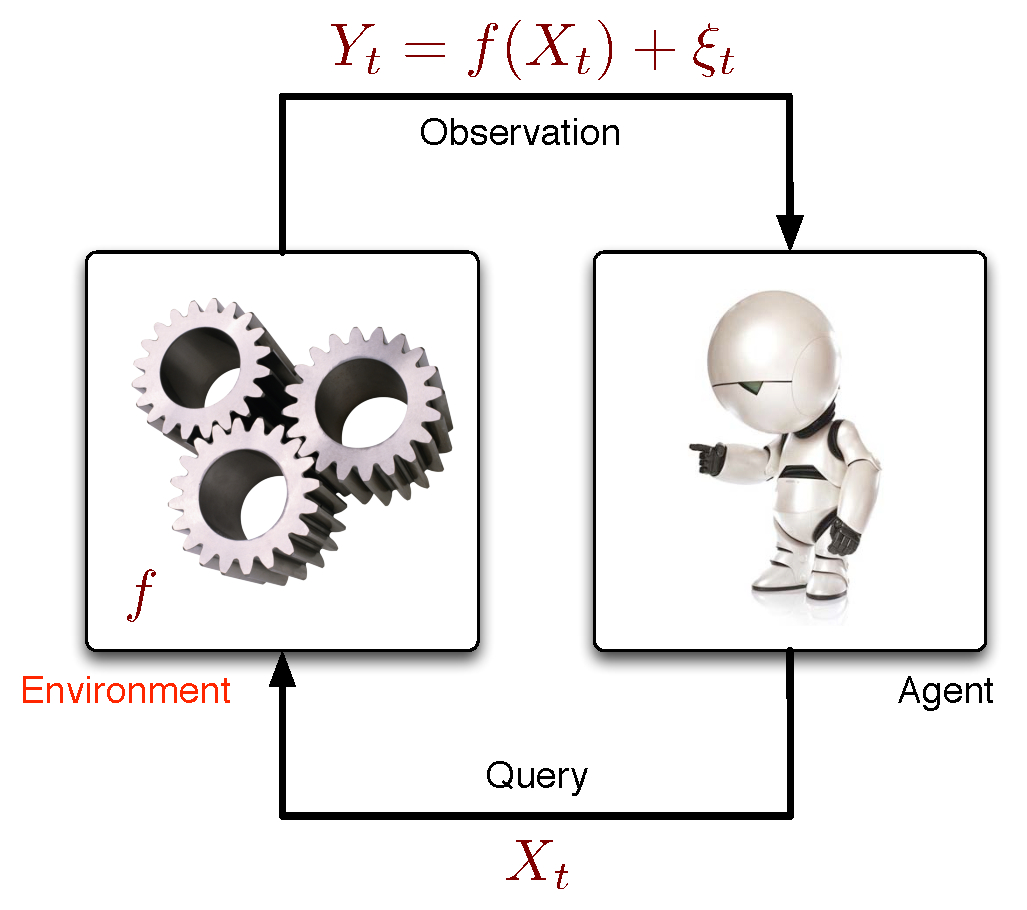
\includegraphics[width=\linewidth]{Interaction} 
\end{minipage} &
\begin{minipage}{0.4\textwidth}
Assume $f$ convex (and smooth etc)\\
{\color{red!80!black} Goal:} Find a near-minimizer of $f$ using $n>0$ queries!
\\
\end{minipage} 
\end{tabular}

 \textbf{How fast can the optimization error}\\[1.5ex]
		$\bm{\Delta_n = \EE{f(X_n) }- \inf_{x\in \cK} f(x)}$\\[1.5ex]
\textbf{decrease with $n$?}
%\vspace{-5ex}
}
%----------------------------------------------------------------------------------------


%----------------------------------------------------------------------------------------
%	SUBCLASSES
%----------------------------------------------------------------------------------------

\headerbox{Subclasses of Problems}{name=subclasses,column=0, below = problems}{
\begin{tabular}[b]{cc}
\begin{minipage}{0.55\textwidth}
\textbf{Curviness}: 
%	\begin{align*}
%	D_f(x,y)\doteq f(x)- \left\{ f(y) + \ip{\nabla f(y),x-y} \right\}.
%	\end{align*}
	
	Smoothness: \\
	$
	D_f(w,v) \le \frac{L}{2} \norm{w-v}^2\,.
	$
	
	Strong convexity:\\
	$
	D_f(w,v) \ge \frac{\mu}{2} \norm{w-v}^2\,.
	$
\end{minipage} &
\begin{minipage}{0.35\textwidth}
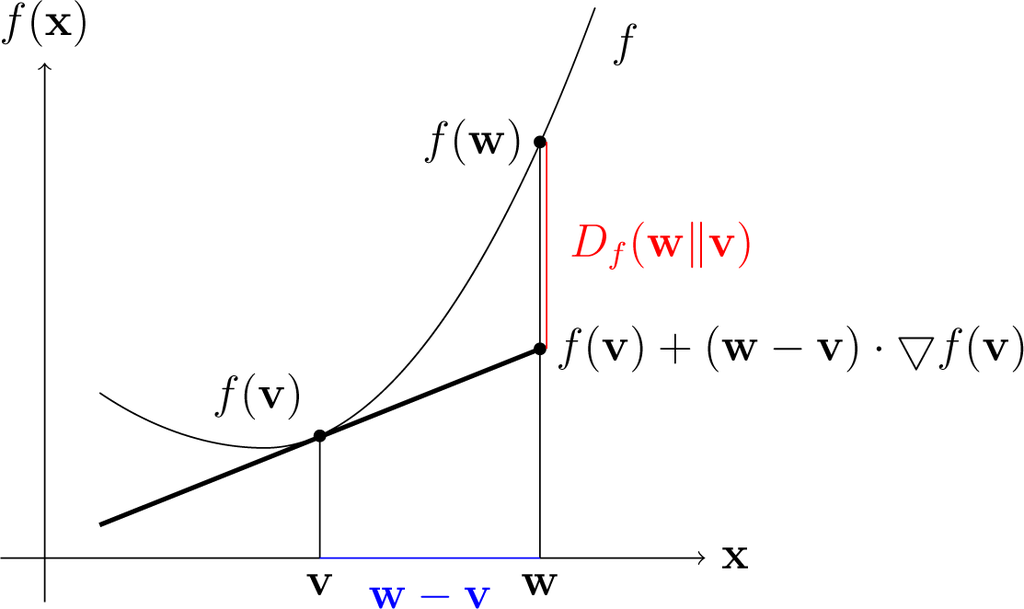
\includegraphics[width=\linewidth]{entropy-16-06338f2-1024} 
\end{minipage}
\end{tabular}

\vspace{1ex}
	\textbf{Noisy} Bandit Feedback:
	
	Recall: $y = f(x) + \xi$, $\EE{y} = \EE{F(x,\xi)}$.
	\begin{itemize}\compresslist
	\item[(A1)] \textbf{\textit{\color{blue}``Uncontrolled noise''}}: $F(x,\xi)$ can be obtained at any point. 
	\item[(A2)] \textbf{\textit{\color{blue}``Controlled noise''}}: $\xi$  can be kept fixed between queries. 
	\end{itemize}
	
}
%----------------------------------------------------------------------------------------

%----------------------------------------------------------------------------------------
%	STATE-OF-THE-ART
%----------------------------------------------------------------------------------------

\headerbox{State of the Art}{name=state_of_the_art,column=0,below=subclasses}{
Controlled Noise: $\Delta_n \leq C\sqrt{d^2/n}$.

Optimal! Let's talk about the uncontrolled case.
\\[1ex]
Ellipsoid method and relatives:
\begin{itemize}\compresslist
\item  Agarwal et al. (2013) --  $\color{blue}\sqrt{d^{33}/n}$.
\item Liang et al. (2014) -- $\color{blue}\sqrt{d^{14}/n}$.
\end{itemize}

Gradient methods:
\begin{itemize}\compresslist
\item Convex: $\color{blue}\left( d^2/n \right)^{1/4}$.
\item Smooth: $\color{blue}\left( d^2/n \right)^{1/3}$.
\item Smooth + Strongly Convex: $\color{red}\sqrt{d^2/n}$
\end{itemize}

Lower Bound: $\color{red}\sqrt{d^2/n}$
\begin{center}
\tikz[baseline]{
            \node[trapezium,trapezium left angle=90,
  trapezium right angle=90, fill=orange!10,anchor=base] (t1)
            {\makecell{
\large \textbf{Big Gaps: Can we do better}\\
\large \textbf{using a ``clever" gradient method?}
}};}	
\end{center}
 
}
%----------------------------------------------------------------------------------------

%----------------------------------------------------------------------------------------
%	ORACLES
%----------------------------------------------------------------------------------------

\headerbox{Gradient Estimation Oracles}{name=oracles,column=1,span = 2}{
\begin{center}
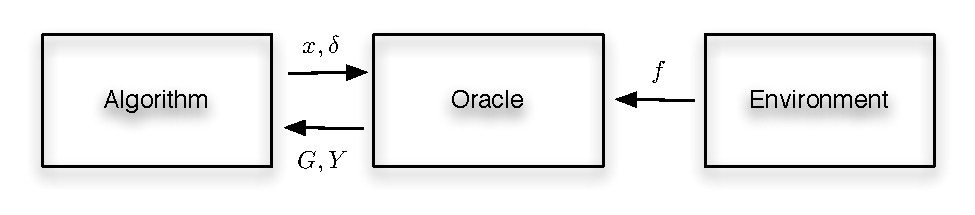
\includegraphics[width=0.8\textwidth]{oracle0}


1. \textbf{Bias}: $\norm{ \EE{G}  - \nabla f(x)  }_* \le c_1(\delta) $; \quad and  \quad
2. \textbf{Second moment}: $\EE{\norm{ G  }_*^2} \le c_2(\delta)$.\\[1ex]

Polynomial oracle: $c_1(\delta) = C_1 \delta^p$, $c_2(\delta) = C_2 \delta^{-q}$, $p,q>0$.

Controlled noise: $c_1(\delta) = C_1\delta^2$, $c_2(\delta) = C_2$.
\quad
Uncontrolled noise:  $c_1(\delta) = C_1\delta^2$, $c_2(\delta) = C_2 \delta^{-2}$.
\end{center}
}
%----------------------------------------------------------------------------------------

%----------------------------------------------------------------------------------------
%	GRADIENT
%----------------------------------------------------------------------------------------

\headerbox{Gradient Estimates}{name=gradient,column=1,span = 2, below=oracles}{
\begin{multicols}{2}
Two-sided Differences -- Noisy Feedback:\\[0.8ex]
$
	G_i = \frac{1}{2\delta} \left\lbrace \left( f(x+\delta e_i)+\xi_i^+\right) - \left( f(x-\delta e_i)+\xi_i^- \right) \right\rbrace
	$\\[0.8ex]
	where $i=1,\cdots,d$.
	
	Assumption: $\EE{\xi^\pm}=0$, $\EE{(\xi^\pm)^2}\leq \sigma^2<\infty$.
	
	Note: $G_i = g_i+\frac{\xi_i^+ - \xi_i^-}{2\delta}$, $\EE{G_i}=g_i$. Hence:

	\textbf{\color{red}bias}:  $ \norm{\EE{G}-\nabla f(x)} = O(\sqrt{d}\color{red}\delta^2\color{black})$ \\
	 \textbf{\color{red}second moment}: $ \EE{G_i^2}=g_i^2+\frac{2\sigma^2}{4\delta^2}$\\
	 \textit{Controlled}: $\EE{\norm{G}^2}=\norm{g}^2$.\\
	 \textit{Uncontrolled}:  $\EE{\norm{G}^2}=\norm{g}^2+O(\dfrac{d}{\color{red}\delta^2})$.
	 
	 
	 General two-point \& one-point estimates:
	 \begin{center}
\tikz[baseline]{
            \node[trapezium,trapezium left angle=90,
  trapezium right angle=90, fill=yellow!20,anchor=base] (t1)
            {\makecell{
$
G = \frac{ (f(x+U)+\xi^+) - (f(x-U)+\xi^-)}{2\delta} V
$\\[0.7ex]
$
G = \frac{ (f(x+U)+\xi^+) }{\delta} V
$
}};}	
\end{center}
	Choose $U,V$ such that $\EE{ V U^\top  } = I$, $\EE{ V } = 0$.
	\vspace{-3ex}
	\begin{itemize} \compresslist
	\item $U \sim \delta\, \cN(0,I)$, 
	         $V = \delta^{-1}\, U$
	\item $U \sim \delta\, \mathrm{Unif}(\mathbb{S}_d)$, 
			 $V =d \delta^{-1}\,  U$
    \item $U_i \sim \delta\, \mathrm{Rademacher}(\pm 1)$, 
			 $V = \delta^{-1} \,U$
	\end{itemize}
	\vspace{-1ex}
	\textbf{Does it matter which of these we select?\\ Not really:}\\
	Bias: $O(\delta^2)$, second moment: $O(1)$ or $O(\delta^{-2})$.
	  
\end{multicols}
}
%----------------------------------------------------------------------------------------

%----------------------------------------------------------------------------------------
%	UPPER BOUND
%----------------------------------------------------------------------------------------

\headerbox{Upper Bound}{name=upper_bound,column=1, below=gradient,bottomaligned=state_of_the_art}{

\textbf{Theorem 1}: 
Consider the Mirror Descent algorithm with a $(c_1,c_2)$, $(p,q)$ polynomial oracle, $\alpha$-strongly convex regularizer $\cR$.
Then:

\begin{center}
\tikz[baseline]{
            \node[trapezium,trapezium left angle=90,
  trapezium right angle=90, fill=green!20,anchor=base] (t1)
            {\makecell{
            $
\Delta_n(\F_{L,0},\mathrm{MD},c_1,c_2 ) 
= O( n^{- \frac{p}{2p+q} } )
$\\[0.7ex]
$
\Delta_n(\F_{L,\mu},\mathrm{MD},c_1,c_2 ) 
= O( n^{- \frac{p}{p+q} } )
$
}};}	
\end{center}


\textbf{Can we get an \color{red}{$n^{-1/2}$} \color{black}rate?}\\
\textbf{Yes}, if $p/(2p+q)\ge 1/2$ vs. $p/(p+q)\ge 1/2$.\\
First holds iff \color{red}$q=0$\color{black}. Second holds iff \color{red}$p\ge q$\color{black}.\\

%\textit{Uncontrolled noise}: \\
%under smoothness $p=q=2$. \\
%For $\F_{L,\mu}$ we get $O(n^{-1/2})$ as Hazan and Levy (2014).\\
%For $\F_{L,0}$ we get $O(n^{-1/3})$ as Saha and Tewari (2011).\\[0.7ex]
%
%\textit{Controlled noise}: \\
%under smoothness $p=2$, $q=0$.\\
%For $\F_{L,\mu}$ we get $O(1/n)$ as Nesterov (2011).\\
%For $\F_{L,0}$ we get $O(n^{-1/2})$ as Duchi et al (2015).
Recover state-of-the-art results:
\begin{center}
\begin{tabular}{l l l}
\toprule
 & $\F_{L,\mu}$ & $\F_{L,0}$\\
\midrule
\textit{Uncontrolled noise} & $O(n^{-1/2})$ & $O(n^{-1/3})$ \\
\textit{Controlled noise} & $O(1/n)$ & $O(n^{-1/2})$ \\
\bottomrule
\end{tabular}
\end{center}

}
%----------------------------------------------------------------------------------------

%----------------------------------------------------------------------------------------
%	LOWER BOUND
%----------------------------------------------------------------------------------------

\headerbox{Lower Bound}{name=lower_bound,column=2, below=gradient}{

\textbf{Theorem 2}: 
$\cK\subset \R^d$ convex, closed, with  $\{+1,-1\}^d\subset \cK$, $n$ large enough.
For any algorithm $\mathrm{A}$ that observes $n$ random elements from a  $(p,q)$ polynomial oracle, we have
\begin{center}
\tikz[baseline]{
            \node[trapezium,trapezium left angle=90,
  trapezium right angle=90, fill=green!20,anchor=base] (t1)
            {\makecell{
            $
\Delta_n(\F_{L,0},\mathrm{A},c_1,c_2 ) = \Omega( n^{-\frac{p}{2p+q}})
$\\[0.7ex]
$
\Delta_n(\F_{L,1},\mathrm{A},c_1,c_2 )  = \Omega(  n^{-\frac{2p}{2p+q}})
$
}};}	
\end{center}

The lower bound for $\F_{L,0}$ is tight, for $\F_{L,1}$ it is weak.\\[1ex]

\textbf{\textsc{Idea:}} \\
Construct two loss functions, whose noisy gradient estimates are so close that they can NOT be distinguished.\\

Choose the convex relaxation of $\epsilon \left| x-v \right|$ for $v \in \{-1,+1\}$:
\begin{align*}
f_v(x) :=\epsilon\left( x-v\right)+2\epsilon^2 \ln\left(1+e^{-\frac{x-v}{\epsilon}}  \right)\,,
\end{align*}
which is $0.5$-smooth.
}
%----------------------------------------------------------------------------------------

%----------------------------------------------------------------------------------------
%	PROOF
%----------------------------------------------------------------------------------------

\headerbox{Proof Sketch}{name=proof,column=0, below=state_of_the_art,span=2}{
\begin{multicols}{2}
Define $\F_{L,0}$ comprised of $f_+$ and $f_-$.
\begin{center}
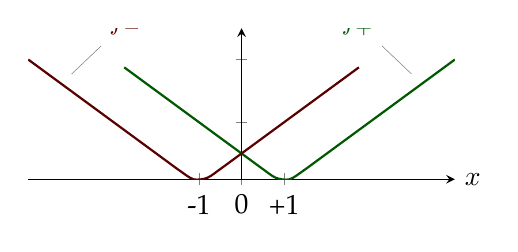
\begin{tikzpicture}
   \begin{axis}[width=7cm,height=3.5cm,
          %  grid = major,         
            axis y line=middle,
            axis x line=bottom,
						xlabel={$x$},
						every axis x label/.style={at={(current axis.right of origin)},anchor=west},
						ymax=0.5,
						xtick={-1,0,1},
            xticklabels={-1,0,+1},
            yticklabels=\empty
            ]
           \addplot[domain=-2.75:5, green!35!black, thick,smooth] 
              {0.1*(x-1) + 2*0.01*ln(1+exp(-10*(x-1)))} node [pos=0.9,pin={135:$f_+$}] {} ; 
            \addplot[domain=-5:2.75, red!35!black,thick,smooth] 
              {0.1*(x+1) + 2*0.01*ln(1+exp(-10*(x+1)))} node [pos=0.1,pin={45:$f_-$}] {} ; 
   \end{axis}
   \end{tikzpicture}
\end{center}

\begin{center}
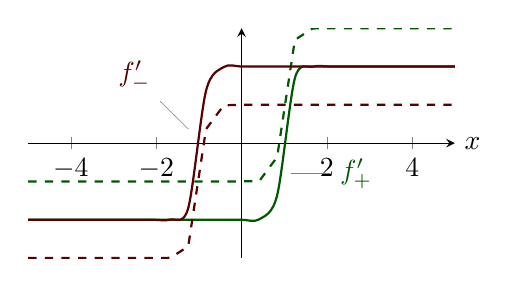
\begin{tikzpicture}
   \begin{axis}[width=7cm,height=4.5cm,
          %  grid = major,         
            axis y line=middle,
            axis x line=middle,
						xlabel={$x$},
						every axis x label/.style={at={(current axis.right of origin)},anchor=west},
            yticklabels=\empty
            ]
           \addplot[domain=-5:5, green!35!black, thick,smooth] 
              {0.1*(1-exp(-10*(x-1)))/(1+exp(-10*(x-1)))} node [pos=0.59,pin={0:$f'_+$}] {}; 
            \addplot[domain=-5:5, green!35!black, thick,dashed] 
              {0.1*(1-exp(-10*(x-1)))/(1+exp(-10*(x-1)))+0.05} ; 
            \addplot[domain=-5:5, red!35!black,thick,smooth] 
              {0.1*(1-exp(-10*(x+1)))/(1+exp(-10*(x+1)))} node [pos=0.4,pin={135:$f'_-$}] {}; 
              \addplot[domain=-5:5, red!35!black,thick,dashed] 
              {0.1*(1-exp(-10*(x+1)))/(1+exp(-10*(x+1)))-0.05};
   \end{axis}
   \end{tikzpicture}
\end{center}
The noisy oracle $\gamma_v$ (dashed line) shifts the gradient (smooth line) by $c_1(\delta)$,  defined as
\begin{align*}
 \gamma_v(x,\delta) = \epsilon \,\dfrac{1-e^{-\frac{x-v}{\epsilon}}}{1+e^{-\frac{x-v}{\epsilon}}} - v\, \min(\epsilon,C_1 \delta^p) + \xi_\delta.
\end{align*}
We get
$
\left| \gamma_+(x,\delta)-\gamma_-(x,\delta)\right|<2(\epsilon-C_1\delta^p)_+ 
$.

The minimax error $\Delta_n^{*}$ is lower bound by 
\begin{align*}
\Delta_n^{*}  \ge & \inf_{\A} \dfrac{\epsilon}{2}\,  \P(\hat X_n V < 0), \\
  \ge &\dfrac{\epsilon}{2} \left(1 - \sqrt{
    n}  \dfrac{ \sup_{\delta>0} (\epsilon-C_1\delta^p)_+\delta^{q/2}}{C_2}
  \right)
\end{align*}
Choosing $\epsilon$ that maximizes the bound gives the result.

\end{multicols}
}
%----------------------------------------------------------------------------------------

%----------------------------------------------------------------------------------------
%	CONCLUSION
%----------------------------------------------------------------------------------------

\headerbox{Conclusions}{name=conclusions,column=2, below=lower_bound}{
To get the optimal $O(n^{-1/2})$ rate for $\F_{L,0}$  with uncontrolled noise,
one of the following must be done:
\begin{enumerate}\compresslist
\item An oracle with $q=0$ (constant second moment bound) must be designed.
\item 
\remove{An algorithm that makes better use of the gradient estimates must be designed.}
\item Some extra properties of gradient estimates must be exploited beyond bias/variance.
\end{enumerate}

}
%----------------------------------------------------------------------------------------

\end{poster}

\end{document}